\documentclass[a4paper,10pt]{article}
\usepackage[utf8]{inputenc}
\usepackage{subcaption}
\usepackage{amsmath}
\usepackage{pgfplots}
\usepackage{float}
\usepackage[parfill]{parskip}
\usepackage{siunitx}
\sisetup{detect-all}

%opening
\title{Měření teplotního součinitele délkové roztažnosti}
\author{Tomáš Kysela}
\date{04/10/2022}

\begin{document}

\maketitle

\section{Použité veličiny}

\begin{tabular}{l l l}
 $l$ & délka měřeného prvku & [\si{\meter}]\\
 $a_i$ & parametr proložení křivkou & \\
 $t$ & teplota & [\si{\celsius}]
\end{tabular}

\section{Známé hodnoty}

\begin{tabular}{l l}
 $L = (600 \pm 1) \si{\milli\meter}$ & délka měřeného vzorku \\
\end{tabular}

\section{Výpočet teplotní součinitele délkové roztažnosti}
\subsection{Naměřené hodnoty}
\begin{equation}
 \Delta l_i = l_i-l_0
\end{equation}
\begin{table}[!ht]
    \centering
    \begin{tabular}{c||c|c|c||c|c|c}
         & \multicolumn{3}{c||}{Mosaz} & \multicolumn{3}{c}{Hliník}\\ \hline
        $i$ & $t_i [\si{\celsius}]$ & $l_i [\si{\milli\meter}]$ & $\Delta l_i [\si{\milli\meter}]$ & $t_i [\si{\celsius}]$ & $l_i [\si{\milli\meter}]$ & $\Delta l_i [\si{\milli\meter}]$\\ \hline\hline
        0 & 24.20 & 0.15 & 0.00 & 27.4 & 0.05 & 0.00\\ \hline
        1 & 31.80 & 0.23 & 0.08 & 31.2 & 0.11 & 0.06\\ \hline
        2 & 36.10 & 0.29 & 0.14 & 35.9 & 0.17 & 0.12\\ \hline
        3 & 40.40 & 0.33 & 0.18 & 41.7 & 0.25 & 0.20\\ \hline
        4 & 46.00 & 0.39 & 0.24 & 46.2 & 0.31 & 0.26\\ \hline
        5 & 50.30 & 0.43 & 0.28 & 49.7 & 0.36 & 0.31\\ \hline
        6 & 56.10 & 0.50 & 0.35 & 56.3 & 0.44 & 0.39\\ \hline
        7 & 61.10 & 0.55 & 0.40 & 60.5 & 0.51 & 0.46
    \end{tabular}
\end{table}

\subsection{Proložení přímkou metodou nejmenších čtverců}
Po proležení dostáváme hodnoty $a_0 = -0.2593$, $a_1 = 0.0108$ pro mosaz a $a_0 = -0.3696$, $a_1 = 0.0136$ pro hliník.

\begin{figure}[H]
\centering
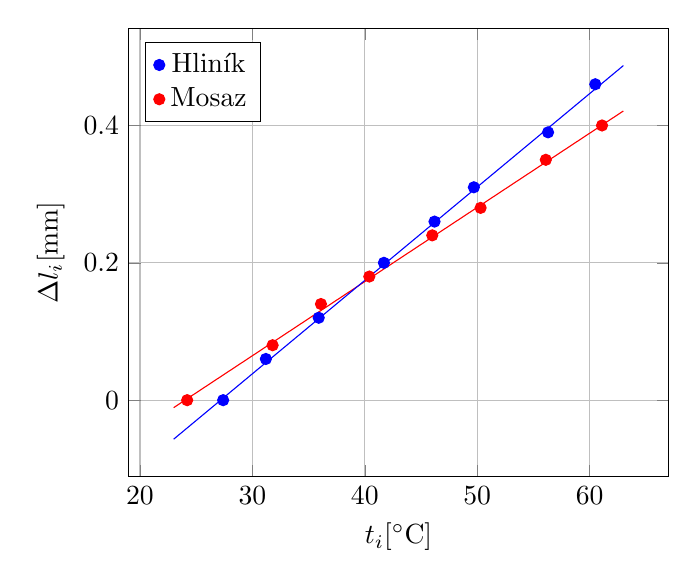
\begin{tikzpicture}
\begin{axis}[
xlabel = {$t_i [\si{\celsius}]$},
ylabel = {$\Delta l_i[\si{\milli\meter}]$},
grid = both,
legend pos=north west,
]
\addplot [
color = blue,
mark = *,
only marks
] coordinates {
(27.4,0.00)
(31.2,0.06)
(35.9,0.12)
(41.7,0.20)
(46.2,0.26)
(49.7,0.31)
(56.3,0.39)
(60.5,0.46)
};
\addlegendentry{Hliník}

\addplot [
color = red,
mark = *,
only marks
] coordinates {
(24.20,0.00)
(31.80,0.08)
(36.10,0.14)
(40.40,0.18)
(46.00,0.24)
(50.30,0.28)
(56.10,0.35)
(61.10,0.40)
};
\addlegendentry{Mosaz}

\addplot [
domain = 23:63,
color = red,
] {0.0108*x-0.2593};

\addplot [
domain = 23:63,
color = blue,
] {0.0136*x-0.3696};
\end{axis}
\end{tikzpicture}
\end{figure}

\subsection{Výpočet součinitele teplotní roztažnosti}
\begin{gather*}
\alpha = \frac{a_1}{L} \\
\\
\alpha_{Mosaz} = \frac{a_{1 Mosaz}}{L} = \frac{0.0108}{600} = 1.8 \cdot 10^{-5} \si{\per\kelvin}\\
\\
\alpha_{Hlinik} = \frac{a_{1 Hlinik}}{L} = \frac{0.0136}{600} = 2.2667 \cdot 10^{-5} \si{\per\kelvin}
\end{gather*}

\subsection{Výpočet nejistot}
\begin{gather*}
 u(L) = \pm1 \si{\milli\meter} \\
 \\
 u(a_{1 Mosaz}) = 0.00015 \\
 \\
 u(a_{1 Hlinik}) = 0.00015\\
 \\
 u(\alpha) = \sqrt{(\frac{1}{L} u(a_1))^2 + (-\frac{a_1}{L^2} u(L))^2}\\
 \\
 u(\alpha_{Mosaz}) = \sqrt{(\frac{1}{600} \cdot 0.00015)^2 + (-\frac{0.0108}{600^2} \cdot 1)^2} = 2.518 \cdot 10^{-7}\\
 u(\alpha_{Hlinik}) = \sqrt{(\frac{1}{600} \cdot 0.00015)^2 + (-\frac{0.0136}{600^2} \cdot 1)^2} = 2.528 \cdot 10^{-7}\\
\end{gather*}

\section{Závěr}
Změřili jsme součinitel teplotní roztažnosti pro mosaz a pro hliník. U mosazy nám vyšel $(1.800 \pm 0.025) \cdot 10^{-5} \si{\per\kelvin}$, což je od tabulkové hodnoty $1.9 \cdot 10^{-5} \si{\per\kelvin}$  odlišné o 5\%. Pro hliník to poté vyšlo $(2.267 \pm 0.025) \cdot 10^{-5} \si{\per\kelvin}$, což je od tabulkové hodnoty $2.3 \cdot 10^{-5} \si{\per\kelvin}$  odlišné o 1\%.
\end{document}
